%%%%%%%%%%%%%%%%%%%%%%%%%%%%%%%%%%%%%%%%%
% Writing Project Poster
% 
% April 12, 2017
%
% Paul Harmon
% Montana State University 
% 
%
%%%%%%%%%%%%%%%%%%%%%%%%%%%%%%%%%%%%%%%%%

%----------------------------------------------------------------------------------------
%	PACKAGES AND OTHER DOCUMENT CONFIGURATIONS
%----------------------------------------------------------------------------------------

\documentclass[a0,portrait]{a0poster}

\usepackage{multicol} % This is so we can have multiple columns of text side-by-side
\columnsep=100pt % This is the amount of white space between the columns in the poster
\columnseprule=3pt % This is the thickness of the black line between the columns in the poster

\usepackage[svgnames]{xcolor} % Specify colors by their 'svgnames', for a full list of all colors available see here: http://www.latextemplates.com/svgnames-colors
\usepackage{subcaption}
\usepackage{grffile}
\usepackage{times} % Use the times font
%\usepackage{palatino} % Uncomment to use the Palatino font

\usepackage{graphicx} % Required for including images
\graphicspath{{figures/}} % Location of the graphics files
\usepackage{booktabs} % Top and bottom rules for table
\usepackage[font=small,labelfont=bf]{caption} % Required for specifying captions to tables and figures
\usepackage{amsfonts, amsmath, amsthm, amssymb} % For math fonts, symbols and environments
\usepackage{wrapfig} % Allows wrapping text around tables and figures
\usepackage{caption}


\begin{document} 

%----------------------------------------------------------------------------------------
%	POSTER HEADER 
%----------------------------------------------------------------------------------------

% The header is divided into two boxes:
% The first is 75% wide and houses the title, subtitle, names, university/organization and contact information
% The second is 25% wide and houses a logo for your university/organization or a photo of you
% The widths of these boxes can be easily edited to accommodate your content as you see fit

\begin{minipage}[b]{0.99\linewidth}
	\centering
\veryHuge \color{NavyBlue} \textbf{Demystifying the Carnegie Classifications} \color{Black}\\ % Title
\Huge\textit{A Sensitivity Analysis}\\[2cm] % Subtitle
\huge \textbf{Paul Harmon}\\[0.5cm] % Author(s)
\huge Montana State University Department of Mathematical Sciences and the Office of Planning and Analysis\\[0.4cm] % University/organization

\end{minipage}
%
%\begin{minipage}[b]{0.25\linewidth}
%\includegraphics[width=10cm]{C:/Users/Paul/Documents/MontanaStateLogo.png}\\
%\end{minipage}
%
\vspace{1cm} % A bit of extra whitespace between the header and poster content

%----------------------------------------------------------------------------------------

\begin{multicols}{2} % This is how many columns your poster will be broken into, a portrait poster is generally split into 2 columns

%----------------------------------------------------------------------------------------
%	ABSTRACT
%----------------------------------------------------------------------------------------

\color{DarkSlateGray} % Navy color for the abstract

\begin{abstract}
The Carnegie Classifications of Institutions are used to compare like institutions in higher education. In 2015, the most recent update of the Carnegie Classifications was released, with Montana State University (MSU) moving from the category of "Highest Research Activity - R1" to the category of "Higher Research Activity - R2."  The classification system of doctoral granting institutions is based on two separate indices calculated using principal components analysis. The first index is based on a set of aggregate covariates and the other on a set of per-capita metrics. 
This analysis re-creates the calculation of the classifications and examines how sensitive they are to changes in the underlying characteristics of a given institution. I analyze how MSU would look in the Carnegie Classifications given changes to each single metric and introduce an application for interactive modeling of multidimensional changes. Based on this analysis, adding at least one social science PhD along with increasing STEM and non-STEM expenditures would help to move MSU towards the R1 status, but getting across the threshold may require changes that are not feasible.    
\end{abstract}

%----------------------------------------------------------------------------------------
%	INTRODUCTION
%----------------------------------------------------------------------------------------

\color{SaddleBrown} % SaddleBrown color for the introduction

\section*{Introduction: The Carnegie Classifications}

Since its initial publication in 1973, the Carnegie Classifications of Institutions of Higher Education have been updated seven times (1976, 1987, 1994, 2000, 2005, 2010, and 2015). They are intended to be used by higher education institutional researchers to identify other schools which are similar in research characteristics so that meaningful comparisons can be made. They are unfortunately often mistaken as a system designed to rank institutional quality; however, the classifications of each institution are not meant to identify schools as being better or worse than institutions in other classifications. \\

In 2015, the Center for Postsecondary Research at the Indiana University School of Education took over the formulation of the classifications. When the 2015 updates were released, Montana State University - among a cohort of several institutions - moved from the "Highest Research Activity" to the "Higher Research Activity" category. I recreated the Carnegie Classifications as part of this analysis. Further, I analyzed the sensitivity to minor perturbations in the underlying indices used to calculate each score for in order to determine which variables most strongly affect the score for a given institution.  Moreover, I created an app that demonstrates where Montana State would end up relative to the other institutions in the dataset if it experienced these slight marginal changes. 

%----------------------------------------------------------------------------------------
%	OBJECTIVES
%----------------------------------------------------------------------------------------

%Include a picture of the Carnegie Classifications
\begin{center}\vspace{1cm}
	\includegraphics[width=0.65\linewidth]{C:/Users/Paul/Documents/Carnegie Classifications/"CC2015".pdf}
	\captionof{figure}{\color{DarkSlateGray} The 2015 Carnegie Classifications. Montana State was classified in the R2: Higher Research Activity group.}
\end{center}\vspace{1cm}

%
%
%Talk about the Carnegie Classifications as a whole:
% Calculating indices, then talk about how they are calculated
%
\color{DarkSlateGray}
\section*{Aggregate and Per-Capita Indices of Research Performance}

\subsection*{Weighted Averages from Principal Components Analysis}

The Aggregate and Per-Capita Indices are based on weighted averages of the number of doctorates awarded, staff size, and expenditures: \\
\small
\begin{eqnarray}
 Ag_i = .37HumD_i + .27StemD_i + .39SocSciD_i + .27OtherD_i + .40StemExp_i + .38NonStem_i + .33ResStaff_i 
\label{eqn:Aggregate Index}
\end{eqnarray}
\\
\begin{eqnarray}
PerCapita_i = \frac{.637StemExp_i + .643NonStem_i + .423ResStaff_i}{FacultySize_i} 
\end{eqnarray}
\\
These indices are each based on a separate Principal Component Analyses of the above variables. The Aggregate index is a one-variable dimension reduction from a 7 variable dataset; the Per-Capita index is a one-variable dimension reduction from a 3 variable set. The Aggregate Index explains 70\% of the variation in the underlying variables; the Per-Capita Index explains 71\%. 

\section*{How are the classifications calculated?}

\begin{enumerate}
\item Each variable is ranked from smallest to largest. Ties are all assigned the minimum rank.
\item Two Principal Components Analyses are fit on the ranked data.
\item An Aggregate and Per-Capita Index are calculated from the first Principal Component of each PCA.
\item The indices are rescaled and new Aggregate Index is plotted against the new Per-Capita Index to create Figure 1.
\item Arcs are drawn with arbitrary radii to define breakpoints between categories.
 
\end{enumerate}

\subsection*{Why Rank the Data?}
Counts of PhDs awarded, expenditures, and research staff/faculty sizes tend to be positively skewed. For instance, Johns Hopkins spent over 2 billion dollars on STEM expenditures in 2015!  Ranking the data prior to classification increases separation between institutions at the low end and decreases separation between institutions with large variable values. 

 \begin{center}\vspace{1cm}
 	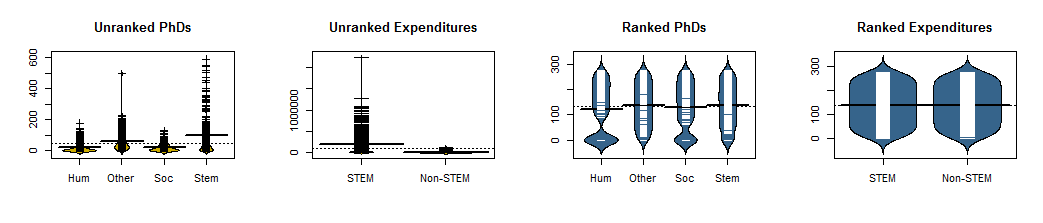
\includegraphics[width=0.95\linewidth]{C:/Users/Paul/Documents/Carnegie Classifications/RankedData.png}
 	\captionof{figure}{\color{DarkSlateGray} Data were ranked prior to using PCA. Ranking mitigated the problem caused by institutions that either spend a lot of money or award unusually large numbers of PhDs. Beanplots (Kampstra, 2008) display the mean as wide lines and observations for each school as narrow lines. }
 \end{center}\vspace{1cm}
 

%----------------------------------------------------------------------------------------
%	RESULTS 
%----------------------------------------------------------------------------------------
\color{DarkSlateGray}
\section*{Single Metric Movement for MSU}
If we tried to move by adjusting just a single variable, it would be nearly impossible for Montana State to get to the R1 category.
  
\begin{center}
	\centering

		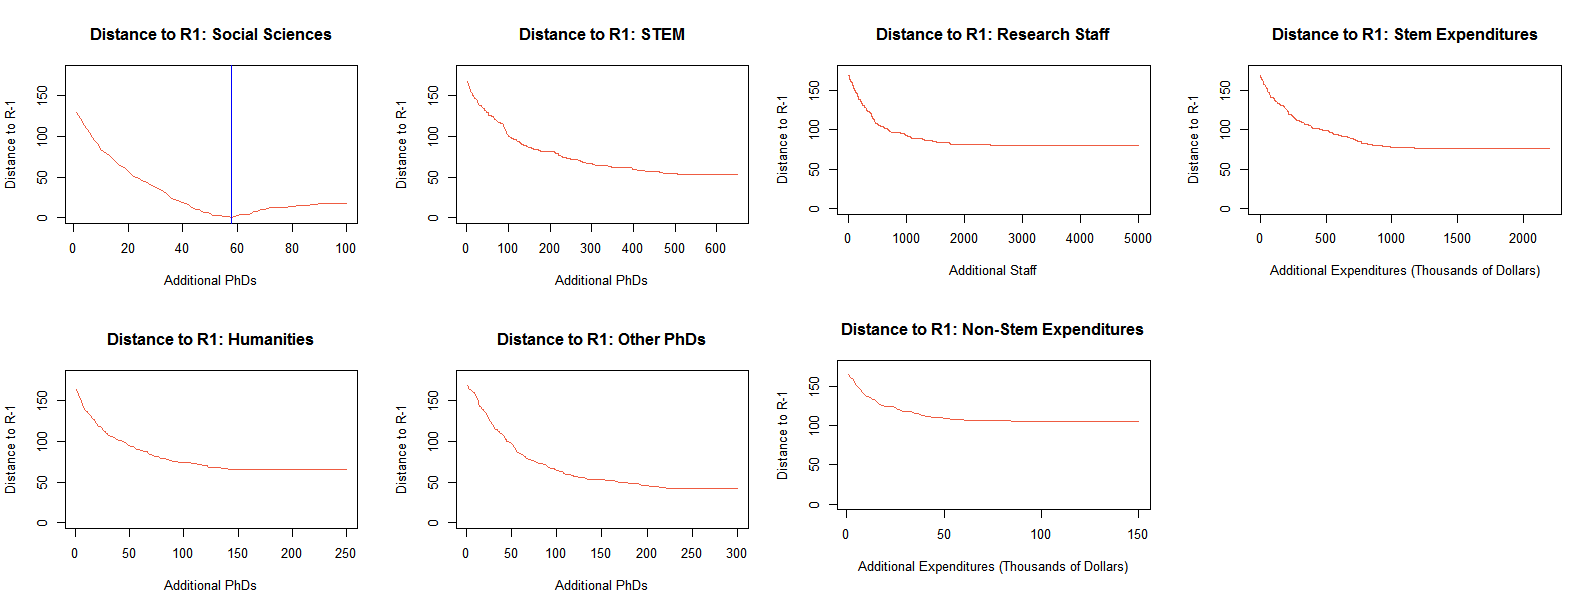
\includegraphics[height = 13 cm] {C:/Users/Paul/Documents/Carnegie Classifications/AllDistances.png}
\captionof{figure}{\color{DarkSlateGray}Increasing Social Science PhD counts can get MSU closer to R1 status, but increasing other PhD counts, expenditures, or research staff size will not get us across the border.}
\end{center}



\color{DarkSlateGray}

\section*{Multi-Dimensional Movement - Shiny App}

In order to assess movement on multiple variables simultaneously, I created an application that recalculates the Carnegie Classifications given different inputs. By focusing on addressing multiple inputs, we can find different paths to R1 status. \textbf{Test different scenarios for Montana State with the application on your phone or a computer}. 
\begin{center}
		
\includegraphics[width=5cm]{C:/Users/Paul/Documents/Carnegie Classifications/CCQRcode.png}\\
	\captionof{figure}{\color{DarkSlateGray} Scan this QR Code to access the Carnegie Classifications App on your phone!}
\end{center}







%----------------------------------------------------------------------------------------
%	CONCLUSIONS
%----------------------------------------------------------------------------------------

\color{SaddleBrown} % SaddleBrown color for the conclusions to make them stand out

\section*{Conclusions}

\subsection*{How do we compare with R1 Schools?}
Results indicate that Montana State produces per-capita research at a high level; however, compared to the R1 schools, we are much smaller on the aggregate levels. Although we are not far from the nearest R1 institutions, MSU produces fewer PhDs and spends less on research than the typical R1 school. 

% Matplot comparing Montana State to R1 Schools
\begin{center}
	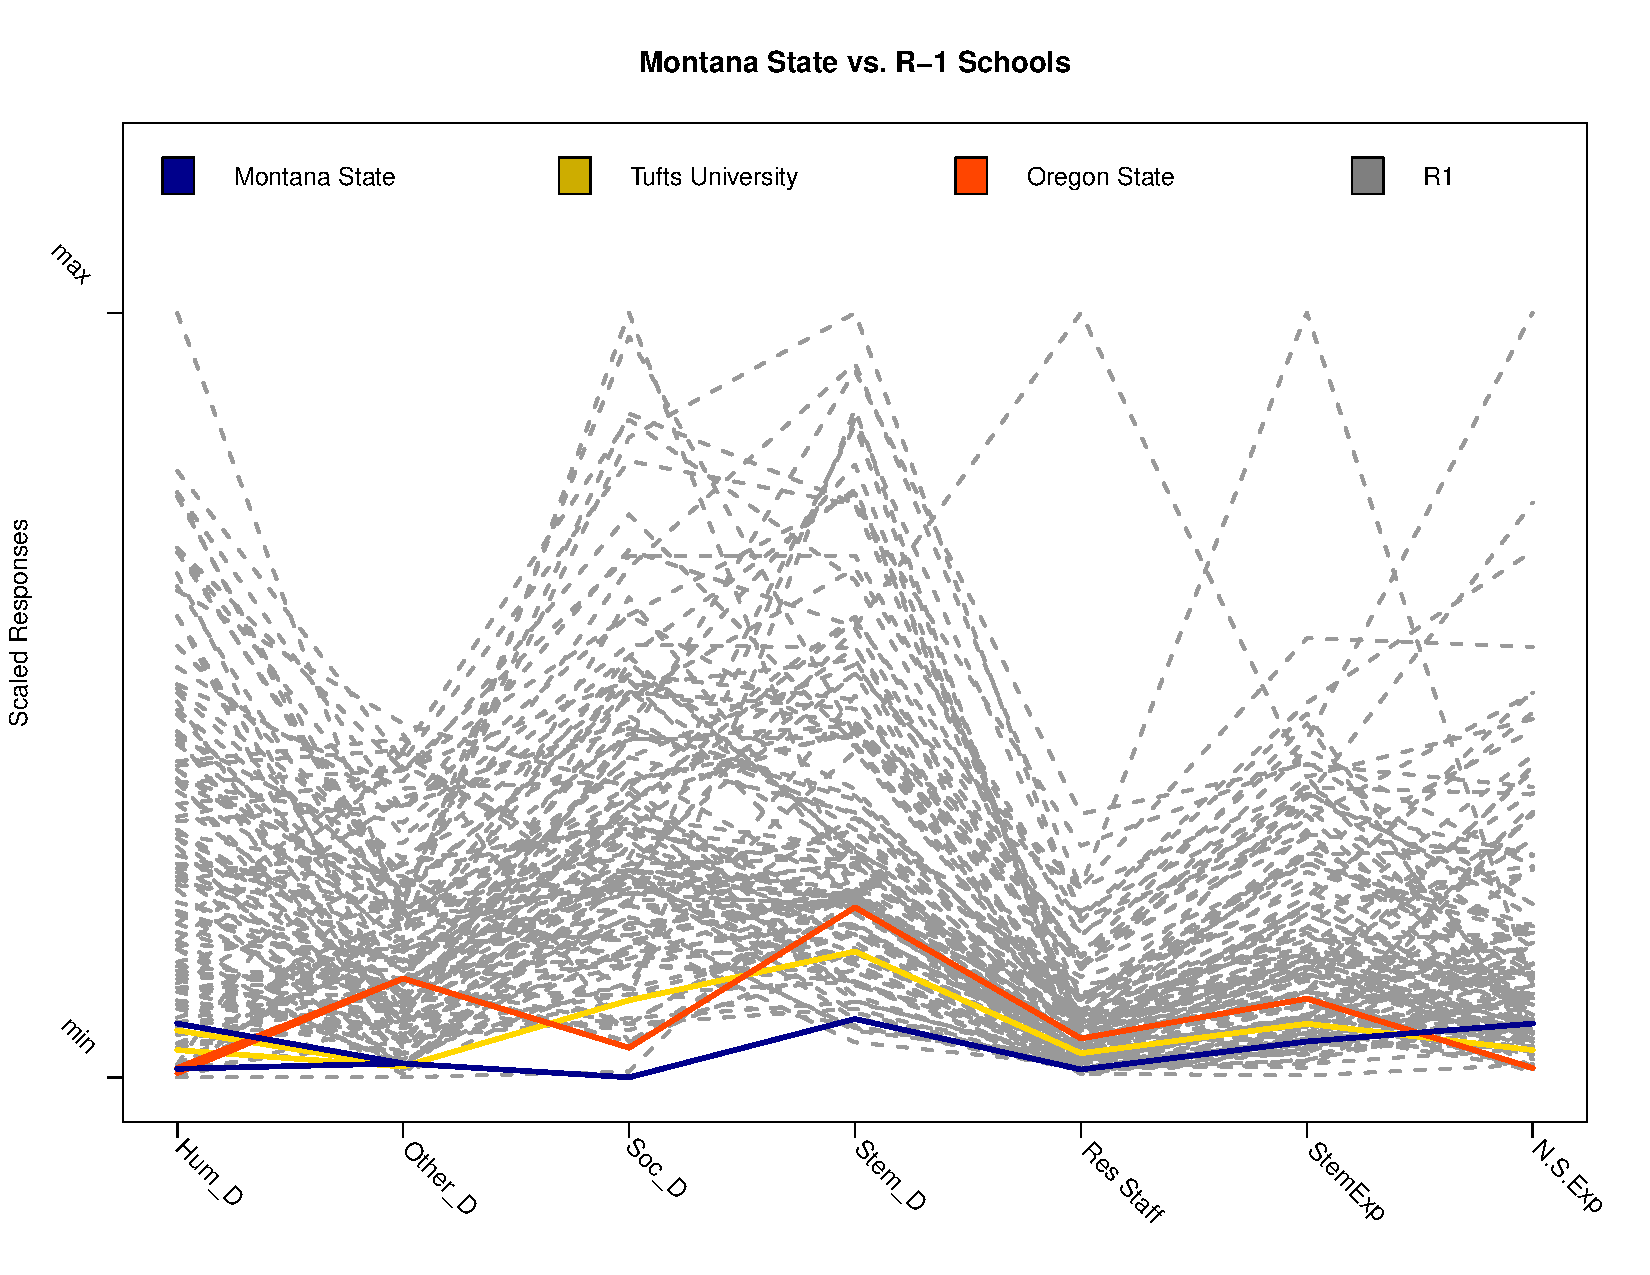
\includegraphics[width=25cm]{C:/Users/Paul/Documents/Carnegie Classifications/r1skools.pdf}\\
	\captionof{figure}{\color{DarkSlateGray} Montana State compared to the R1 schools on all Carnegie Classification variables. Tufts University and Oregon State University are MSU's nearest R1 neighbors in the classifications.}
\end{center}


\color{SaddleBrown}
\subsection*{Should we prioritize move towards R1?}
 % Set the color back to DarkSlateGray for the rest of the content
\begin{itemize}
	\item Moving towards R1 necessitates growth in PhDs, Research Staff and Expenditures
	\item Maintaining our status is just as important as moving towards R1. Drops in the number of  PhDs or expenditures can result in moving towards R-3 
	\item The delineations between the doctoral Carnegie Classifications (where the arcs are drawn) are \textbf{subjective}. Comparing student profiles, graduation rates, and other metrics of student performance indicates that we fit in better with R2 institutions than R1 schools. 
\end{itemize}

\subsection*{Did the Carnegie Classifications Change?}
In short, no. The way that the Carnegie Classifications did not change radically between the 2010 and 2015 updates. However, some minor changes were made in the 2015 update: 
\begin{itemize}
	\item Delineations between groups were no longer hand-drawn; rather, the lines between groups are circles with radii 984 and 489. 
	\item Universities were no longer moved across the border to R1 by hand. 
\end{itemize}


\color{DarkSlateGray}


\begin{thebibliography}{9}
\bibitem{PersonalCommmunication}
Borden, V. (March 2017). \textit{Personal Communication}.


\bibitem{EandH}
Everitt, B., and Hothorn, T. (2011). \textit{An introduction to applied multivariate analysis with R}. Berlin: Springer.
\bibitem{Elements}
Friedman, J., Hastie, T., and Tibshirani, R. (2009). \textit{The Elements of Statistical Learning: Data Mining, Inference, and Prediction} (2nd ed.). Springer.
\bibitem{beanplot}
Kampstra, P. (2008). \textit{Beanplot: A Boxplot Alternative for Visual Comparison of Distributions}. Journal of
Statistical Software, Code Snippets 28(1). 1-9. \texttt{http://www.jstatsoft.org/v28/c01/}.
\bibitem{mcclintick}
McClintick, W. (2016). \textit{Carnegie Sensitivity Analysis: Moving from R2 to R1}. Poster Presentation at Rocky Mountain Association of Institutional Research Conference.

\end{thebibliography}




%----------------------------------------------------------------------------------------
%	ACKNOWLEDGEMENTS
%----------------------------------------------------------------------------------------

\section*{Acknowledgments}

I would like to thank Dr. Mark Greenwood with the Department of Mathematical Sciences. I would also like to thank Dr. Chris Fastnow, Dr. Ian Godwin, and Rebecca Belou with the Office of Planning and Analysis. Finally, Dr. Victor Borden with the Center for Indiana University Center for Postsecondary Research and Chair of the Carnegie Classifications for being willing to answer my many questions. 

%----------------------------------------------------------------------------------------

\end{multicols}
\end{document}